\documentclass[titlepage]{article}

\usepackage[margin=1in]{geometry}
% some more shit for the title
\usepackage[T1]{fontenc}
\usepackage{babel}

% Tables and stopping them from displaying in a different section
\usepackage{booktabs}
\usepackage[section]{placeins}

% for inserting images into the document, setting file path, and allowing rotation of inserted images 
\usepackage{graphicx}
\graphicspath{ {./images/} }
\usepackage{rotating}
\usepackage[table]{xcolor}
% mostly just for putting text in math equations
\usepackage{amsmath}
% for aligning the text to the left
\usepackage[document]{ragged2e}

% for inserting hyperlinks in the document, use \url{url} or \href{url}{text}
\usepackage{hyperref}
\usepackage{calligra}
\usepackage[T1]{fontenc}
\usepackage{siunitx}
\usepackage{caption}
\usepackage{multirow}
\usepackage[export]{adjustbox}
\usepackage{tikz}
\usepackage{pgfplots}
\pgfplotsset{soldot/.style={color=black,only marks,mark=*},
	             holdot/.style={color=black,fill=white,only marks,mark=*},
		                  compat=1.12}
\usepackage{paracol}

\begin{document}
\title{\textbf{Lab 6: RC Circuits}}
\author{
    Zachary Pouska\\
    \texttt{001103193}\\
    \and
    Natalie Tran \\ 
    \texttt{000698629}\\ \\
} 

\date{PHYS 236 | Fall 2022\\
Date performed: 11/02/2022}


	\maketitle



	\section{Purpose}
	\section{Theory}	
	\section{Experiment Analysis}


    $$V_c = \varepsilon \left( 1- e^{-\frac{t}{\tau}} \right)  | \div $$
    



	\section{Procedure}




	\section{Data and Graphs}
	\subsection{Part I: Calculate the value of the time constant}
		The measured value of capacitance of the the capacitor is
		\(\mathbf{ 104.7\pmb{\mu} F }\) \\
		The measured value of the resistor using the DMM is
	\(\pmb{0.987 M\Omega} \)
		\begin{table}[ht!]
			\rowcolors{2}{gray!10}{gray!40}
			\caption*{\textbf{Calculated Time Constants}}
			\centering
			\begin{tabular}{c|c|c}
				$\tau_{measured}$ (sec) & $\tau_{nominal}$ (sec) & \% Error \\
				\hline
				103.34 & 100 & 3.34
			\end{tabular}
		\end{table}

	\subsection{Part II: Charging the capacitor } 
	\begin{minipage}[h]{0.5\textwidth}
		\rowcolors{2}{gray!10}{gray!40}
		\textbf{Voltage v Time for Charging}
		\vspace{1cm}
		\centering
		\begin{tabular}{c|c}
			Time (sec) & Voltage (V) \\
			\hline
			5   & 0.198  \\
			10  & 0.361  \\
			15  & 0.494  \\
			20  & 0.626  \\
			25  & 0.757  \\
			30  & 0.868  \\
			35  & 0.993  \\
			40  & 1.087  \\
			45  & 1.189  \\
			50  & 1.287  \\
			55  & 1.375  \\
			60  & 1.455  \\
			65  & 1.549  \\
			70  & 1.617  \\
			75  & 1.698  \\
			80  & 1.772  \\
			85  & 1.832  \\
			90  & 1.9    \\
			100 & 2.033  \\
			110 & 2.136  \\
			120 & 2.245  \\
			130 & 2.343  \\
			140 & 2.43   \\
			150 & 2.514  \\
			160 & 2.594  \\
			170 & 2.667  \\
			185 & 2.767  \\
			200 & 2.855  \\
			220 & 2.956  \\
			240 & 3.047  \\
			260 & 3.125  \\
			280 & 3.193  \\
			305 & 3.265  \\
			330 & 3.328  \\
			355 & 3.375  \\
			380 & 3.419  \\
			400 & 3.449  \\
			420 & 3.473  \\
			435 & 3.491  \\
			450 & 3.507  \\
			465 & 3.519  \\
			480 & 3.535  \\
			500 & 3.548 \\
			510 & 3.556 \\
			540 & 3.575 \\
			570 & 3.589 \\
			630 & 3.612 \\
			720 & 3.634 \\
			780 & 3.648
		\end{tabular}
		\vspace{14.8cm}
	\end{minipage}
	\begin{minipage}[b]{0.5\textwidth}
		\rowcolors{2}{gray!10}{gray!40}
				\centering
		\textbf{Voltage v Time Linearized}
		\FloatBarrier
				\begin{tabular}{c|c}
					Time (sec) & $-\frac{1}{\tau}$ \\
					\hline
					5   & -0.051  \\
					10  & -0.094  \\
					15  & 0.148   \\
					20  & 0.191   \\
					25  & 0.236   \\
					30  & 0.276   \\
					35  & 0.323   \\
					40  & 0.359   \\
					45  & 0.401   \\
					50  & 0.442   \\
					55  & 0.481   \\
					60  & 0.518   \\
					65  & 0.563   \\
					70  & 0.596   \\
					75  & 0.638   \\
					80  & 0.678   \\
					85  & 0.711   \\
					90  & 0.750   \\
					100 & 0.832   \\
					110 & 0.900   \\
					120 & 0.977   \\
					130 & 1.052   \\
					140 & 1.124   \\
					150 & 1.198   \\
					160 & 1.275   \\
					170 & 1.350   \\
					185 & 1.464   \\
					200 & 1.575   \\
					220 & 1.721   \\
					240 & 1.873   \\
					260 & 2.025   \\
					280 & 2.180   \\
					305 & 2.375   \\
					330 & 2.583   \\
					355 & 2.773   \\
					380 & 2.990   \\
					400 & 3.171   \\
					420 & 3.345   \\
					435 & 3.497   \\
					450 & 3.656   \\
					465 & 3.794   \\
					480 & 4.014  
				\end{tabular}
				\vspace{0.2cm}
			\end{minipage}
			\begin{center}
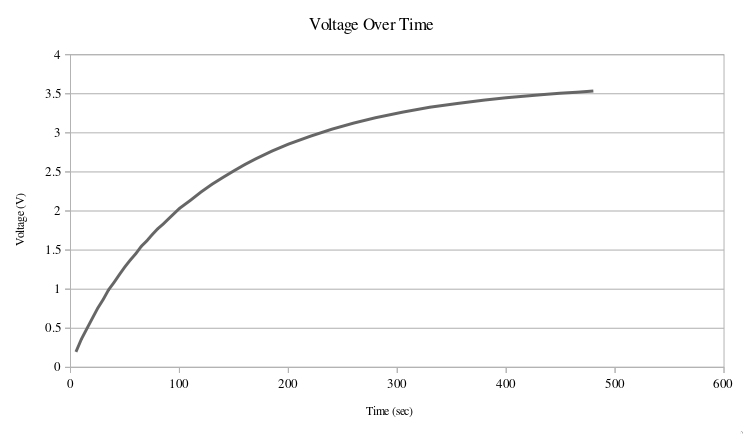
\includegraphics[width=0.9\linewidth,frame]{Voltage-Time.png}
\FloatBarrier
\vspace{1cm}
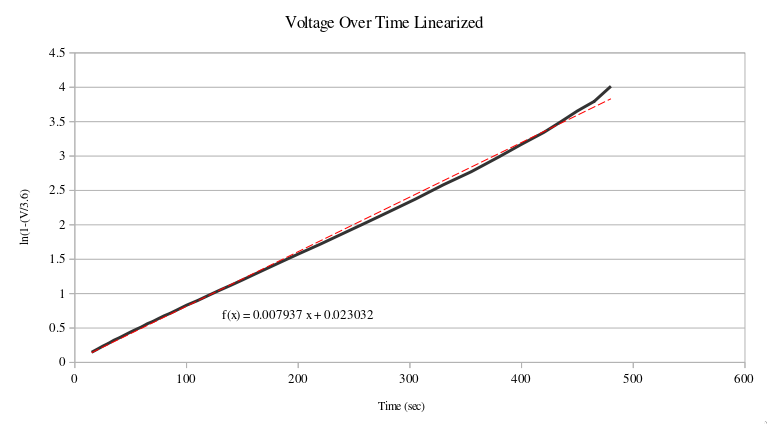
\includegraphics[width=0.9\linewidth,frame]{Voltage-Time-Linear.png}
			\end{center}
			\newpage
	\subsection{Part III: Discharging the capacitor}
			\begin{table}[ht!]
				\rowcolors{2}{gray!10}{gray!40}
				\centering
				\caption*{\textbf{Voltage v Time for Discharging}}
			\begin{tabular}{c|c}
				Time (sec) & Voltage (V)\\
				\hline
				5   & 0.198  \\
				10  & 0.361  \\
				15  & 0.494  \\
				20  & 0.626  \\
				25  & 0.757  \\
				30  & 0.868  \\
				35  & 0.993  \\
				40  & 1.087  \\
				45  & 1.189  \\
				50  & 1.287  \\
				55  & 1.375  \\
				60  & 1.455  \\
				65  & 1.549  \\
				70  & 1.617  \\
				75  & 1.698  \\
				80  & 1.772  \\
				85  & 1.832  \\
				90  & 1.9    \\
				100 & 2.033  \\
				110 & 2.136  \\
				120 & 2.245  \\
				130 & 2.343  \\
				140 & 2.43   \\
				150 & 2.514  \\
				160 & 2.594  \\
				170 & 2.667  \\
				185 & 2.767  \\
				200 & 2.855  \\
				220 & 2.956  \\
				240 & 3.047  \\
				260 & 3.125  \\
				280 & 3.193  \\
				305 & 3.265  \\
				330 & 3.328  \\
				355 & 3.375  \\
				380 & 3.419  \\
				400 & 3.449  \\
				420 & 3.473  \\
				435 & 3.491  \\
				450 & 3.507  \\
				465 & 3.519  \\
				480 & 3.535 
			\end{tabular}
		\end{table}
		\FloatBarrier
		\begin{center}
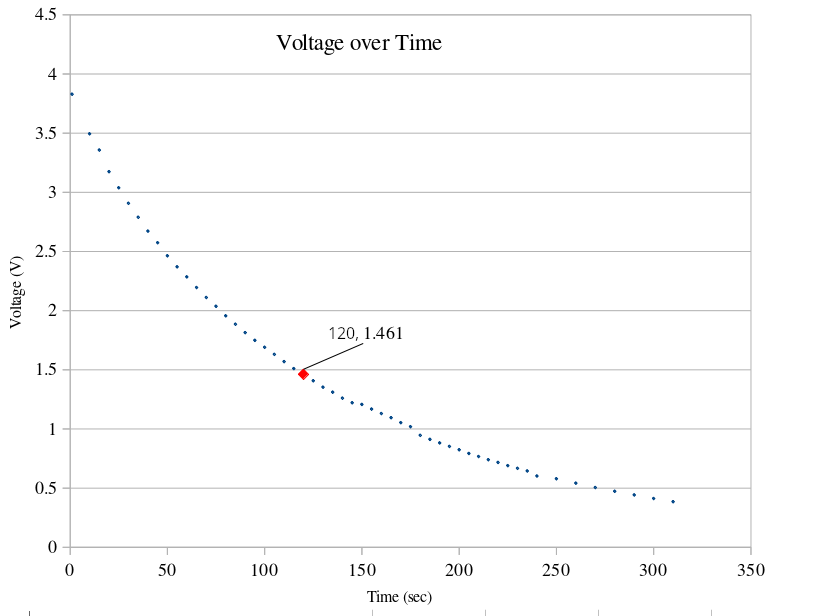
\includegraphics[width=0.9\linewidth,frame]{help.png}
\end{center}
	\subsection{Part IV: Connecting R and C in parallel}
	The voltage read across the resistor with the DMM is \textbf{4.009 V}\\
The voltage read across the capacitor with the DMM is \textbf{4.009 V}\\
	\section{Results}
	\subsection{Part I:Calculate the value of the time constant}
	To calculate the time constant ($\tau$) the resistor is multiplied by the capacitor value via the equation 
	$$\tau = \text{RC}$$
	Substitute the measured values of resistance and capacitance in the equation to recieve the data values stated in Section 5.1.\\
	To calculate the percent error between the expected time constant vs actual time constant created from differing expected resistance and capacitance values, the percent error formula is used
	$$\% error = \frac{|\tau_{measured} - \tau_{nominal}|}{\tau_{nominal}} \times 100$$
	\subsection{Part II: Charging the capacitor}
	In order to linearize the voltage values measured, the following expression is examined:
	$$V_c = \varepsilon \left(1-e^{\frac{-t}{\tau}}\right)$$
	\subsection{Part III: Discharging the capacitor}
	The time constant can be determined by selecting the value of voltage in which it is 37\% of the max voltage (emf). Then, at that point, the time is the time constant. $0.37 \times 4.0$V = $1.48$. The closest point to 1.48 in our graph is 1.461, in which the time is 120 seconds. This means the determined time constant from discharging is 120.
	\subsection{Part IV: Connecting R and C in parallel}
	To calculate the current through the resistor, the equation V = IR is used. Manipulating this equation, current can be found via I = V/R. Using the measured values of resistance and voltage, current can be found as $\frac{4.009V}{0.987M\Omega} = 4.062\mu A$.\\
	The max charge can be calculated using the equation $Q_{max} = C\varepsilon$ substituting values, $104.7\mu F \times 4.009V = 419.7\mu C$
	The energy stored in the capacitor can be found using the equataion $U = \frac{1}{2}C\varepsilon^2$. Substituting values, $\frac{1}{2}104.7\mu F \times 4.009^2 = 841.4\mu J$
	\section{Questions}
    \subsection{Part 4}
    \begin{enumerate}
        \item Do you obtain the same values for the voltage across the resistor and capacitor? Explain.\\ 
            \textbf{Yes! They are in parallel, so the potential difference across each should be the same. If the potential difference wasn’t equal, that wouldn’t make sense, as measuring the potential difference across each one is essentially connecting the multimeter to the same point in the circuit, assuming 0 resistance in the wires.}
        \item Is the current across the resistor zero? Explain.\\ 
            \textbf{No. In the case of the resistor and capacitor being in series, as the capacitor fills up, it blocks the current flow through the resistor. In this configuration, as the capacitor charges more current is simply diverted through the resistor instead of through the capacitor.}



    \end{enumerate}

	\section{Conclusion}

\end{document}
